% Created by tikzDevice version 0.12.3.1 on 2021-09-17 14:35:58
% !TEX encoding = UTF-8 Unicode
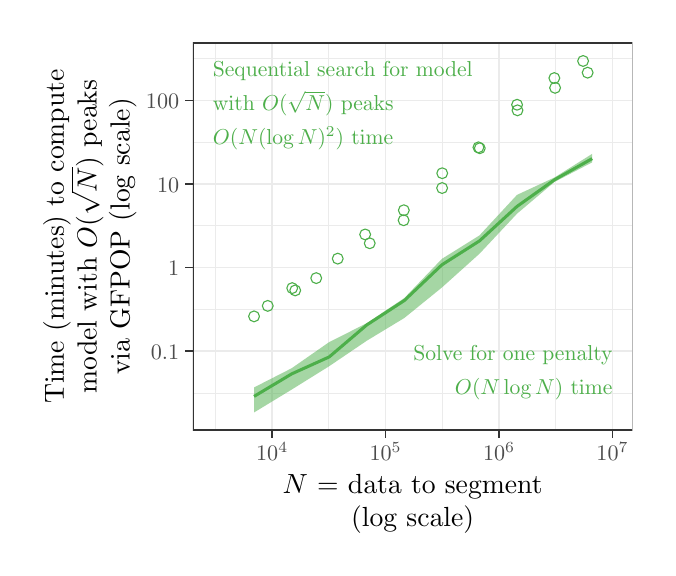
\begin{tikzpicture}[x=1pt,y=1pt]
\definecolor{fillColor}{RGB}{255,255,255}
\path[use as bounding box,fill=fillColor,fill opacity=0.00] (0,0) rectangle (224.04,187.90);
\begin{scope}
\path[clip] (  0.00,  0.00) rectangle (224.04,187.90);
\definecolor{drawColor}{RGB}{255,255,255}
\definecolor{fillColor}{RGB}{255,255,255}

\path[draw=drawColor,line width= 0.6pt,line join=round,line cap=round,fill=fillColor] (  0.00, -0.00) rectangle (224.04,187.90);
\end{scope}
\begin{scope}
\path[clip] ( 59.70, 42.49) rectangle (218.54,182.40);
\definecolor{fillColor}{RGB}{255,255,255}

\path[fill=fillColor] ( 59.70, 42.49) rectangle (218.54,182.40);
\definecolor{drawColor}{gray}{0.92}

\path[draw=drawColor,line width= 0.3pt,line join=round] ( 59.70, 55.91) --
	(218.54, 55.91);

\path[draw=drawColor,line width= 0.3pt,line join=round] ( 59.70, 86.12) --
	(218.54, 86.12);

\path[draw=drawColor,line width= 0.3pt,line join=round] ( 59.70,116.32) --
	(218.54,116.32);

\path[draw=drawColor,line width= 0.3pt,line join=round] ( 59.70,146.53) --
	(218.54,146.53);

\path[draw=drawColor,line width= 0.3pt,line join=round] ( 59.70,176.73) --
	(218.54,176.73);

\path[draw=drawColor,line width= 0.3pt,line join=round] ( 67.85, 42.49) --
	( 67.85,182.40);

\path[draw=drawColor,line width= 0.3pt,line join=round] (108.84, 42.49) --
	(108.84,182.40);

\path[draw=drawColor,line width= 0.3pt,line join=round] (149.83, 42.49) --
	(149.83,182.40);

\path[draw=drawColor,line width= 0.3pt,line join=round] (190.82, 42.49) --
	(190.82,182.40);

\path[draw=drawColor,line width= 0.6pt,line join=round] ( 59.70, 71.02) --
	(218.54, 71.02);

\path[draw=drawColor,line width= 0.6pt,line join=round] ( 59.70,101.22) --
	(218.54,101.22);

\path[draw=drawColor,line width= 0.6pt,line join=round] ( 59.70,131.43) --
	(218.54,131.43);

\path[draw=drawColor,line width= 0.6pt,line join=round] ( 59.70,161.63) --
	(218.54,161.63);

\path[draw=drawColor,line width= 0.6pt,line join=round] ( 88.35, 42.49) --
	( 88.35,182.40);

\path[draw=drawColor,line width= 0.6pt,line join=round] (129.34, 42.49) --
	(129.34,182.40);

\path[draw=drawColor,line width= 0.6pt,line join=round] (170.33, 42.49) --
	(170.33,182.40);

\path[draw=drawColor,line width= 0.6pt,line join=round] (211.32, 42.49) --
	(211.32,182.40);
\definecolor{drawColor}{RGB}{77,175,74}

\node[text=drawColor,anchor=base west,inner sep=0pt, outer sep=0pt, scale=  0.78] at ( 66.92,170.19) {Sequential search for model};

\node[text=drawColor,anchor=base west,inner sep=0pt, outer sep=0pt, scale=  0.78] at ( 66.92,157.90) {with $O(\sqrt N)$ peaks};

\node[text=drawColor,anchor=base west,inner sep=0pt, outer sep=0pt, scale=  0.78] at ( 66.92,145.61) {$O(N(\log N)^2)$ time};

\node[text=drawColor,anchor=base east,inner sep=0pt, outer sep=0pt, scale=  0.78] at (211.32, 67.51) {Solve for one penalty};

\node[text=drawColor,anchor=base east,inner sep=0pt, outer sep=0pt, scale=  0.78] at (211.32, 55.22) {$O(N \log N)$ time};
\definecolor{fillColor}{RGB}{77,175,74}

\path[fill=fillColor,fill opacity=0.50] ( 81.80, 57.90) --
	( 95.37, 64.82) --
	(108.95, 74.28) --
	(122.52, 81.11) --
	(136.10, 90.19) --
	(149.67,104.35) --
	(163.25,112.83) --
	(176.82,127.48) --
	(190.40,133.78) --
	(203.97,142.30) --
	(203.97,139.22) --
	(190.40,132.17) --
	(176.82,120.68) --
	(163.25,106.20) --
	(149.67, 94.00) --
	(136.10, 82.99) --
	(122.52, 74.77) --
	(108.95, 65.57) --
	( 95.37, 57.11) --
	( 81.80, 48.85) --
	cycle;

\path[] ( 81.80, 57.90) --
	( 95.37, 64.82) --
	(108.95, 74.28) --
	(122.52, 81.11) --
	(136.10, 90.19) --
	(149.67,104.35) --
	(163.25,112.83) --
	(176.82,127.48) --
	(190.40,133.78) --
	(203.97,142.30);

\path[] (203.97,139.22) --
	(190.40,132.17) --
	(176.82,120.68) --
	(163.25,106.20) --
	(149.67, 94.00) --
	(136.10, 82.99) --
	(122.52, 74.77) --
	(108.95, 65.57) --
	( 95.37, 57.11) --
	( 81.80, 48.85);

\path[draw=drawColor,line width= 1.1pt,line join=round] ( 81.80, 54.65) --
	( 95.37, 62.78) --
	(108.95, 68.92) --
	(122.52, 80.47) --
	(136.10, 89.30) --
	(149.67,102.20) --
	(163.25,110.84) --
	(176.82,123.30) --
	(190.40,132.96) --
	(203.97,140.58);

\path[draw=drawColor,line width= 0.4pt,line join=round,line cap=round] ( 81.80, 83.58) circle (  1.96);

\path[draw=drawColor,line width= 0.4pt,line join=round,line cap=round] ( 86.75, 87.37) circle (  1.96);

\path[draw=drawColor,line width= 0.4pt,line join=round,line cap=round] ( 95.59, 93.79) circle (  1.96);

\path[draw=drawColor,line width= 0.4pt,line join=round,line cap=round] ( 96.68, 92.96) circle (  1.96);

\path[draw=drawColor,line width= 0.4pt,line join=round,line cap=round] (104.27, 97.40) circle (  1.96);

\path[draw=drawColor,line width= 0.4pt,line join=round,line cap=round] (112.04,104.44) circle (  1.96);

\path[draw=drawColor,line width= 0.4pt,line join=round,line cap=round] (121.95,113.18) circle (  1.96);

\path[draw=drawColor,line width= 0.4pt,line join=round,line cap=round] (123.60,109.99) circle (  1.96);

\path[draw=drawColor,line width= 0.4pt,line join=round,line cap=round] (135.85,118.31) circle (  1.96);

\path[draw=drawColor,line width= 0.4pt,line join=round,line cap=round] (135.92,121.93) circle (  1.96);

\path[draw=drawColor,line width= 0.4pt,line join=round,line cap=round] (149.76,129.95) circle (  1.96);

\path[draw=drawColor,line width= 0.4pt,line join=round,line cap=round] (149.80,135.30) circle (  1.96);

\path[draw=drawColor,line width= 0.4pt,line join=round,line cap=round] (162.88,144.66) circle (  1.96);

\path[draw=drawColor,line width= 0.4pt,line join=round,line cap=round] (163.37,144.33) circle (  1.96);

\path[draw=drawColor,line width= 0.4pt,line join=round,line cap=round] (176.84,160.05) circle (  1.96);

\path[draw=drawColor,line width= 0.4pt,line join=round,line cap=round] (176.99,158.03) circle (  1.96);

\path[draw=drawColor,line width= 0.4pt,line join=round,line cap=round] (190.31,169.69) circle (  1.96);

\path[draw=drawColor,line width= 0.4pt,line join=round,line cap=round] (190.58,166.16) circle (  1.96);

\path[draw=drawColor,line width= 0.4pt,line join=round,line cap=round] (200.70,175.86) circle (  1.96);

\path[draw=drawColor,line width= 0.4pt,line join=round,line cap=round] (202.34,171.64) circle (  1.96);
\definecolor{drawColor}{gray}{0.20}

\path[draw=drawColor,line width= 0.6pt,line join=round,line cap=round] ( 59.70, 42.49) rectangle (218.54,182.40);
\end{scope}
\begin{scope}
\path[clip] (  0.00,  0.00) rectangle (224.04,187.90);
\definecolor{drawColor}{gray}{0.30}

\node[text=drawColor,anchor=base east,inner sep=0pt, outer sep=0pt, scale=  0.80] at ( 54.75, 68.00) {0.1};

\node[text=drawColor,anchor=base east,inner sep=0pt, outer sep=0pt, scale=  0.80] at ( 54.75, 98.20) {1};

\node[text=drawColor,anchor=base east,inner sep=0pt, outer sep=0pt, scale=  0.80] at ( 54.75,128.41) {10};

\node[text=drawColor,anchor=base east,inner sep=0pt, outer sep=0pt, scale=  0.80] at ( 54.75,158.61) {100};
\end{scope}
\begin{scope}
\path[clip] (  0.00,  0.00) rectangle (224.04,187.90);
\definecolor{drawColor}{gray}{0.20}

\path[draw=drawColor,line width= 0.6pt,line join=round] ( 56.95, 71.02) --
	( 59.70, 71.02);

\path[draw=drawColor,line width= 0.6pt,line join=round] ( 56.95,101.22) --
	( 59.70,101.22);

\path[draw=drawColor,line width= 0.6pt,line join=round] ( 56.95,131.43) --
	( 59.70,131.43);

\path[draw=drawColor,line width= 0.6pt,line join=round] ( 56.95,161.63) --
	( 59.70,161.63);
\end{scope}
\begin{scope}
\path[clip] (  0.00,  0.00) rectangle (224.04,187.90);
\definecolor{drawColor}{gray}{0.20}

\path[draw=drawColor,line width= 0.6pt,line join=round] ( 88.35, 39.74) --
	( 88.35, 42.49);

\path[draw=drawColor,line width= 0.6pt,line join=round] (129.34, 39.74) --
	(129.34, 42.49);

\path[draw=drawColor,line width= 0.6pt,line join=round] (170.33, 39.74) --
	(170.33, 42.49);

\path[draw=drawColor,line width= 0.6pt,line join=round] (211.32, 39.74) --
	(211.32, 42.49);
\end{scope}
\begin{scope}
\path[clip] (  0.00,  0.00) rectangle (224.04,187.90);
\definecolor{drawColor}{gray}{0.30}

\node[text=drawColor,anchor=base,inner sep=0pt, outer sep=0pt, scale=  0.80] at ( 88.35, 31.50) {$10^4$};

\node[text=drawColor,anchor=base,inner sep=0pt, outer sep=0pt, scale=  0.80] at (129.34, 31.50) {$10^5$};

\node[text=drawColor,anchor=base,inner sep=0pt, outer sep=0pt, scale=  0.80] at (170.33, 31.50) {$10^6$};

\node[text=drawColor,anchor=base,inner sep=0pt, outer sep=0pt, scale=  0.80] at (211.32, 31.50) {$10^7$};
\end{scope}
\begin{scope}
\path[clip] (  0.00,  0.00) rectangle (224.04,187.90);
\definecolor{drawColor}{RGB}{0,0,0}

\node[text=drawColor,anchor=base,inner sep=0pt, outer sep=0pt, scale=  1.00] at (139.12, 19.51) {$N$ = data to segment};

\node[text=drawColor,anchor=base,inner sep=0pt, outer sep=0pt, scale=  1.00] at (139.12,  7.63) {(log scale)};
\end{scope}
\begin{scope}
\path[clip] (  0.00,  0.00) rectangle (224.04,187.90);
\definecolor{drawColor}{RGB}{0,0,0}

\node[text=drawColor,rotate= 90.00,anchor=base,inner sep=0pt, outer sep=0pt, scale=  1.00] at ( 13.04,112.44) {Time (minutes) to compute};

\node[text=drawColor,rotate= 90.00,anchor=base,inner sep=0pt, outer sep=0pt, scale=  1.00] at ( 24.92,112.44) {     model with $O(\sqrt N)$ peaks};

\node[text=drawColor,rotate= 90.00,anchor=base,inner sep=0pt, outer sep=0pt, scale=  1.00] at ( 36.80,112.44) {     via GFPOP (log scale)};
\end{scope}
\end{tikzpicture}
